\documentclass[a4paper,10pt]{article}
\usepackage{graphicx}
\usepackage{amsmath}
\usepackage{hyperref}
\usepackage{geometry}
\usepackage{natbib}
\usepackage{project}
\usepackage{tikz}
\usepackage{wrapfig}
\usepackage{subcaption}
\usetikzlibrary{positioning, shapes.geometric, arrows}

\geometry{margin=1in}

\title{Interlinked Dynamics: Exploring the Correlations between Chronic Disease Indicators and Specific Death Rates}
\author{Muhammad Ahsan Khan (23491860)}
\date{\today}

\begin{document}
	\maketitle
	
	\section{Questions}
		\begin{itemize}
			\item Are there correlations between chronic disease indicators (e.g., diabetes prevalence) and specific death rates (e.g., due to heart disease)?
			\item What were the leading causes of death each year between 2020 and 2023?
		\end{itemize}
	
	\section{Data Sources}
	\subsection{Descriptions of Data Sources}
	\begin{itemize}
		\item \textbf{Datasource 1: Monthly Provisional Counts of Deaths by Select Causes (2020--2023)}
		
		The dataset includes the total counts of deaths attributed to different causes like heart disease, diabetes, cancer and COVID-19. It provides data spanning both time-related (monthly from 2020 to 2023) and geographic coverage for the United States. \cite{dataset1}
	
	\end{itemize}

	\begin{itemize}
		\item \textbf{Datasource 2: U.S. Chronic Disease Indicators (CDI)} 
		
		The dataset includes information on chronic disease indicators highlighting prevalence rates, demographic distributions and trends over time. By providing the insights of underlying health conditions that are leading to death, this dataset helps in getting a deeper understanding about the factors contributing to deaths. \cite{dataset2}
		
	\end{itemize}
	
	\subsection{Structure and Quality of Data Sources}
	\begin{itemize}
		\item \textbf{Monthly Provisional Counts of Deaths by Select Causes}
		
		The dataset represents the monthly provisional counts of deaths characterized by cause. Each columns represents distinct types of disease associated with the deaths, while the rows display the total death counts with the corresponding dates, months, years and different causes of death (e.g., heart disease, diabetes, cancer). There are a few missing values, but most columns have no missing data. Some columns are empty, however, they are not necessary for the analysis
		\begin{figure}[ht!]
			\centering
			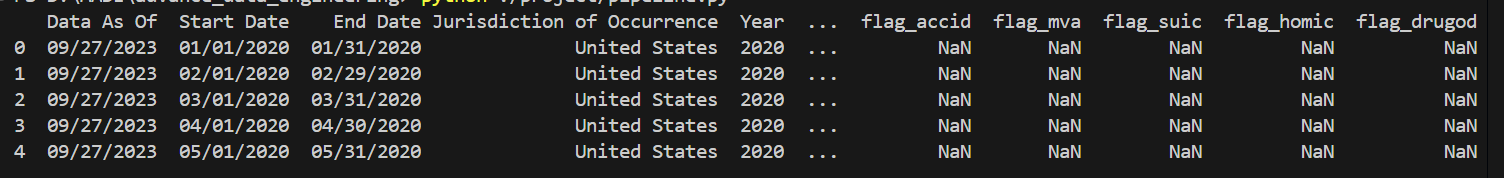
\includegraphics[width=0.9\textwidth]{images/dataset-1.png}
			\caption{First 5 rows of Monthly Provisional Counts of Deaths by Select Causes.}
			\label{fig:dataset1}
		\end{figure}
	\end{itemize}
	\begin{itemize}
		\item \textbf{U.S. Chronic Disease Indicators (CDI)} 
		
		The dataset is represented in tabular format where the rows represents health indicators and columns are grouped by demographics (e.g., gender, race, geographic location). The primary columns in the dataset are year, location, topic (indicator), questions and datavalue. Some columns are empty, however, they are not necessary for the analysis.
		\begin{figure}[ht!]
			\centering
			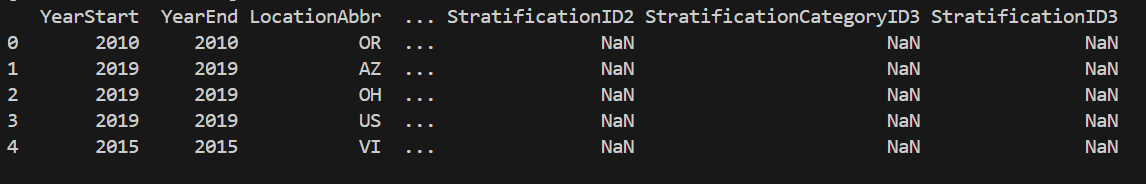
\includegraphics[width=0.9\textwidth]{images/dataset-2.png}
			\caption{First 5 rows of U.S. Chronic Disease Indicators (CDI).}
			\label{fig:dataset2}
		\end{figure}
		
	\end{itemize}

	\subsection{Licenses and Permissions}
	\begin{itemize}
	\item \textbf{Monthly Provisional Counts of Deaths by Select Causes (2020--2023)}
	
	The data is licensed under the \texttt{U.S. Government Work (Public Domain)}. The dataset is publicly available and produce by the U.S. Government. The dataset is free to use, with the only requirement being tp provide proper attribution to the U.S. government. Additionally, to ensure that no logos or other content are used in a way that implies endorsement by the U.S. government. \cite{licenses2}
	\end{itemize}
	
	\begin{itemize}
	\item \textbf{U.S. Chronic Disease Indicators (CDI)} 
		
	This dataset is available for free use under\texttt{Open Database License (ODbL)}. User are required to provide proper attribution to the original source. Additionally, any derived work must be shared under the same license. \cite{licenses1}
		
	\end{itemize}


	\subsection{Data Pipeline}
The data pipeline is developed using Python. It contains three main modules: extract, transform, load. These modules contain the following functionalities.
 
 We start by reading the metadata from a JSON file (\texttt{datasources.json}) to gather information about the data sources like URL, and columns to be removed. The process starts by extracting the data from the URL using the \texttt{CsvExtractor} function, which retrieves the dataset in a CSV. Next, unnecessary columns are removed using the \texttt{DeleteColumns} function, based on the configuration provided in the metadata. If a filtering query is specified for the dataset, the \texttt{FilterRows} function is used to filter the data accordingly. Then, empty values in the dataset are filled using the \texttt{FillEmptyValues} function to ensure completeness. Finally, the transformed dataset is loaded into the SQLite database (\texttt{ChronicHealthTrends.db}) using the \texttt{LoadDfToSqlite} function, storing the data with the appropriate dataset name.
\begin{figure}[h]
	\centering
	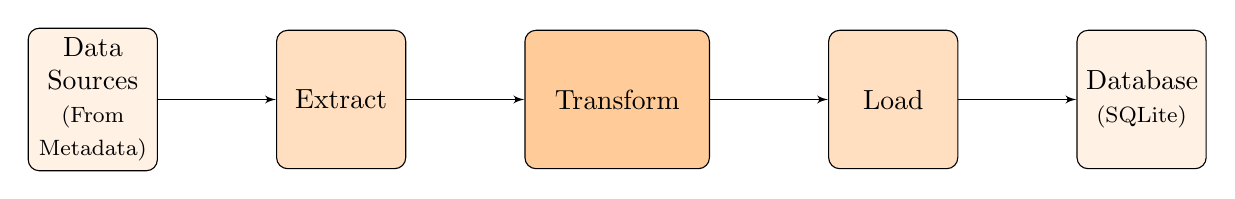
\begin{tikzpicture}[node distance=1.5cm and 1.5cm, auto]
		% Styles
		\tikzstyle{block} = [rectangle, draw, fill=orange!10,
		text width=4em, text centered, rounded corners, minimum height=5em]
		\tikzstyle{bigblock} = [rectangle, draw, fill=orange!25,
		text width=4em, text centered, rounded corners, minimum height=5em]
		\tikzstyle{biggerblock} = [rectangle, draw, fill=orange!40,
		text width=6em, text centered, rounded corners, minimum height=5em]
		\tikzstyle{line} = [draw, -latex', shorten >=0pt, shorten <=0pt]
		
		% Nodes
		\node [block] (sources) {Data Sources \footnotesize(From Metadata)};
		\node [bigblock, right=of sources] (extract) {Extract};
		\node [biggerblock, right=of extract] (transform) {Transform};
		\node [bigblock, right=of transform] (load) {Load};
		\node [block, right=of load] (database) {Database \footnotesize(SQLite)};
		
		% Connections
		\path [line] (sources) -- (extract);
		\path [line] (extract) -- (transform);
		\path [line] (transform) -- (load);
		\path [line] (load) -- (database);
	\end{tikzpicture}
	\caption{ETL Process Diagram}
	\label{fig:etl_process_diagram}
\end{figure}

	
\subsection{Results and Limitations}
The resulting datesets are stored in SQLLite in tabular format as it is the most efficient and reliable way to store collective data. The pipeline can maintain the quality of data. The resultant datasets
\begin{itemize}
	\item fulfill the requirement that is needed to answer the questions.
	\item time domain is overlapping and fitting
	\item ensure format is consistent
\end{itemize}

The datasets on chronic disease indicators and mortality statistics can be compared and analyzed to uncover correlations between chronic health conditions and mortality trends across various demographic and geographic segments. This analysis provides a detailed understanding of the underlying health factors contributing to death rates. However, a limitation exists regarding the granularity of chronic disease data, as it may not provide sufficient specificity directly link certain health indicators to the cause of mortality.






\newpage
\section{Questions}

\subsection{Are there correlations between chronic disease indicators (e.g., diabetes prevalence) and specific death rates (e.g., due to heart disease)?}

\begin{wrapfigure}{r}{0.61\textwidth} % Image aligned to the right
	\centering
	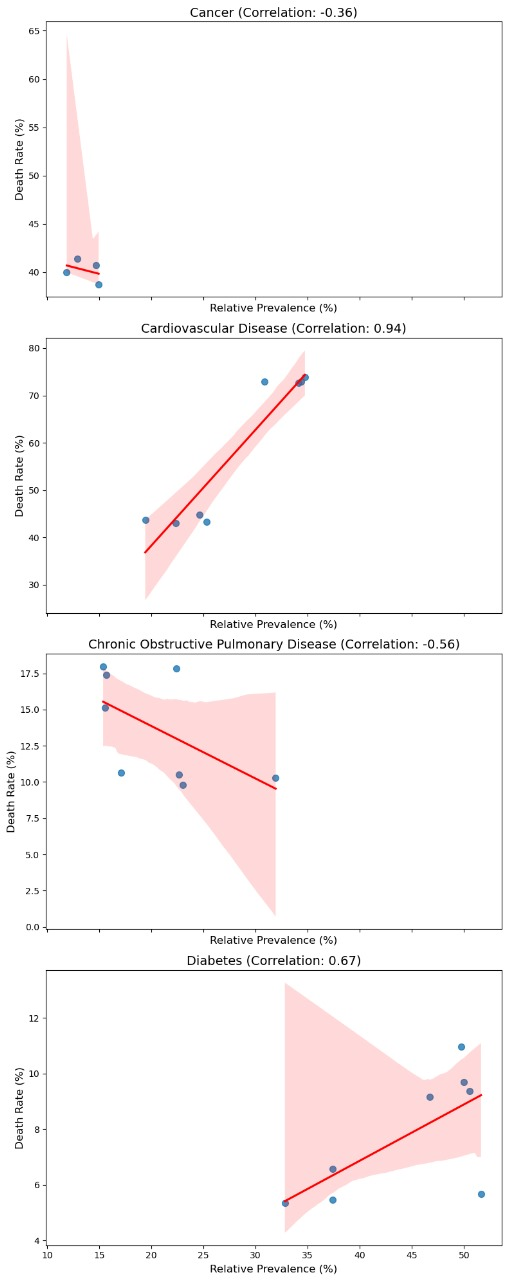
\includegraphics[width=0.38\textwidth]{images/graph-1.png} % Image file added
	\caption{Correlation Between Chronic Disease Relative Prevalence and Death Rates}
	\label{fig:scatterplot}
\end{wrapfigure}

I started by building a data pipeline to handle all the data engineering tasks, ensuring the datasets were clean, organized, and ready for analysis. Once the groundwork was laid, I delved into each dataset, exploring them individually to uncover some fascinating insights. From there, I created scatter plots with regression lines for each chronic disease to better understand the relationship between relative prevalence and death rates. The regression lines helped highlight trends and potential correlations, with steeper slopes indicating stronger relationships. Along the way, I identified data points that significantly deviated from the trendline as potential outliers or exceptions.

The results varied by disease. For diabetes, a moderate positive correlation was observed (correlation: 0.67), indicating that higher relative diabetes prevalence often coincided with higher death rates. Cardiovascular disease exhibited a strong positive correlation (correlation: 0.94), suggesting a significant increase in death rates with higher relative prevalence. In contrast, cancer showed a weak negative correlation (correlation: -0.36), implying that death rates may not align closely with relative prevalence. Chronic Obstructive Pulmonary Disease (COPD) displayed a moderate negative correlation (correlation: -0.56), reflecting some variability in the relationship. For mental health, the correlation was weaker or inconsistent, suggesting that factors beyond relative prevalence may significantly influence related death rates.

\subsection{What were the leading causes of death each year between 2020 and 2023?}

To identify the leading diseases causing death each year between 2020 and 2023, I began by filtering the dataset to focus specifically on these years. The year was extracted from the datetime column to facilitate comparison with integer values representing each year. I then excluded irrelevant columns, such as "Month," "All Cause," and "Natural Cause," focusing only on the columns related to specific causes of death. The death counts for each cause were then aggregated yearly, ensuring the data was numeric and that any missing or invalid values were handled. To highlight the most impactful diseases, I selected the top 5 leading causes of death based on total death counts for each year. Finally, I created a bar plot to visually present the results, grouping the causes by year and using color to distinguish between diseases.

\begin{figure}[ht!]
	\centering
	\begin{subfigure}[t]{0.48\textwidth}
		\centering
		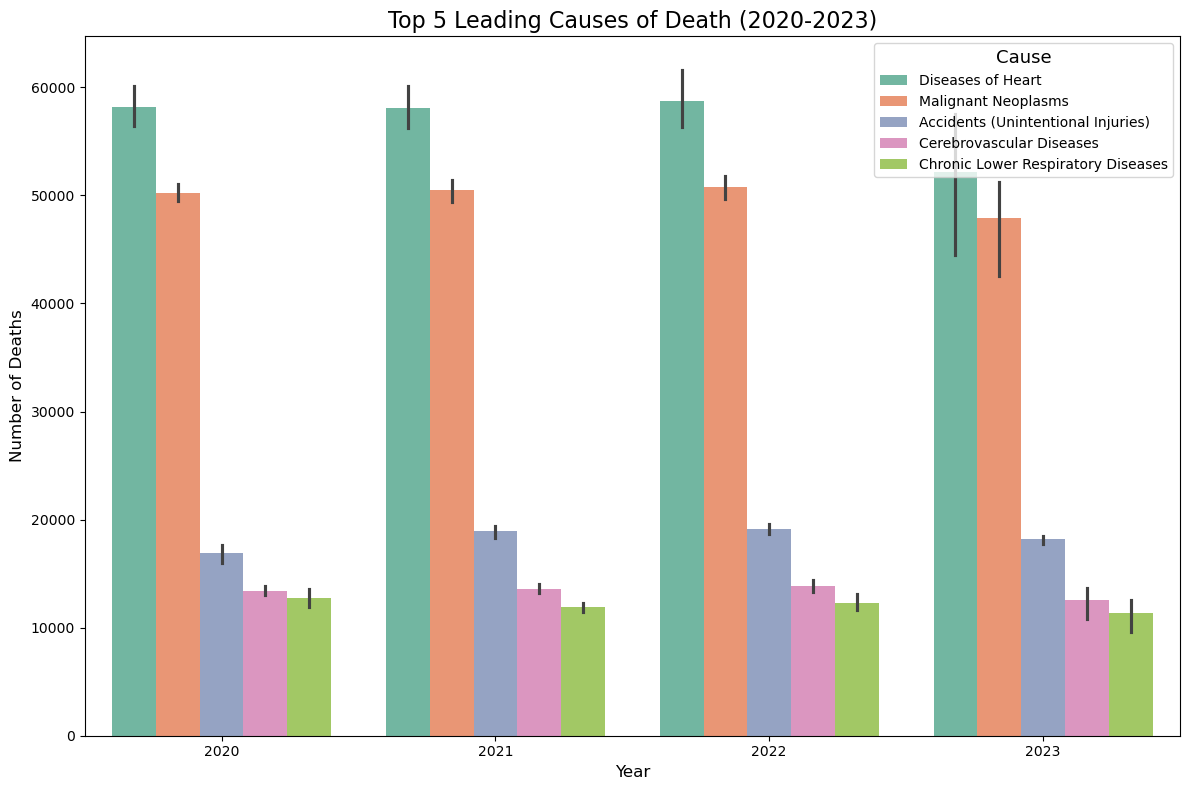
\includegraphics[width=\textwidth]{images/graph-2.png} % Image file added
		\label{fig:comparison-bar}
	\end{subfigure}
	\hfill
	\begin{subfigure}[t]{0.48\textwidth}
		\centering
		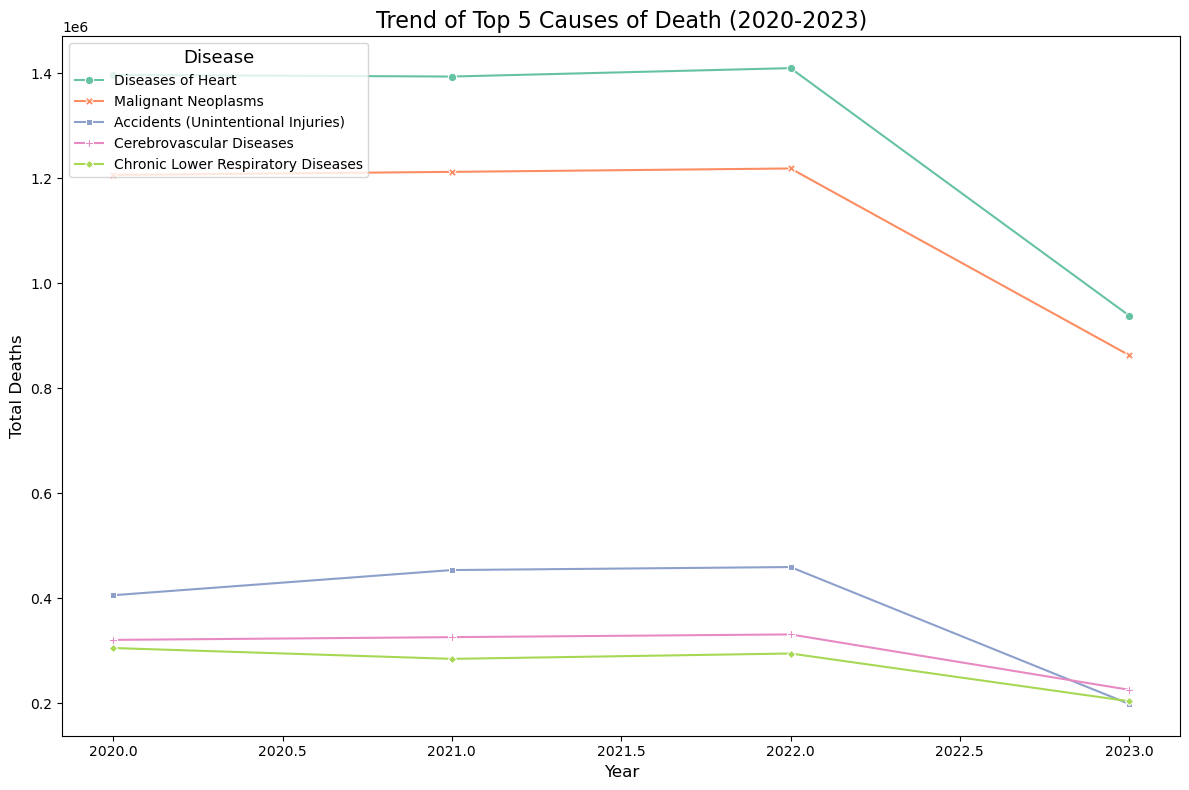
\includegraphics[width=\textwidth]{images/graph-3.png} % Image file added
		\label{fig:comparison-trend}
	\end{subfigure}
	\caption{Comparison of Top Causes of Death and Their Trends (2020-2023)}
\end{figure}

The results, displayed in the graphs, show the top 5 leading causes of death from 2020 to 2023. The bar chart highlights the year-over-year variation in the leading diseases, with some remaining consistent, such as cardiovascular diseases and cancer, while others fluctuated. Chronic diseases like cardiovascular diseases and cancer continued to dominate as leading causes of death throughout the period.

\section{Conclusion}

Yes, there are correlations between chronic disease indicators and specific death rates, but the strength of these correlations varies by disease. Diseases like cardiovascular disease and diabetes exhibit strong positive correlations with death rates, while cancer and mental health show weaker or inconsistent relationships. Additionally, the analysis of the leading causes of death between 2020 and 2023 revealed that while chronic diseases such as cardiovascular disease and cancer consistently remained among the top causes of death, external factors may have influenced year-to-year variations.

\vspace{1em}

The question was partially answered. While correlations between disease prevalence and death rates were identified, causation cannot be inferred from this analysis. The impact of external factors might have influenced the trends observed, making it challenging to isolate the specific contribution of chronic diseases alone. Furthermore, healthcare quality, lifestyle, and demographic factors could also independently influence death rates.

\vspace{1em}

Following are the limitations:
\begin{itemize}
	\item The analysis assumes linear relationships, which may not fully capture more complex patterns or interactions between variables.
	\item The dataset only considers shared years between datasets, which may exclude relevant trends over longer periods.
	\item Outliers and noise in the data were not deeply analyzed, potentially affecting the robustness of the results.
	\item The focus was on the top causes of death, which might overlook important secondary contributors.
\end{itemize}






\bibliographystyle{plain}
\bibliography{references}

\end{document}
